\chapter{Phương pháp giải quyết vấn đề}
Ở chương này chúng tôi trình bày phương pháp tiếp cận gồm lựa chọn các bộ dữ liệu phù hợp cho nghiên cứu, đề xuất mô hình và phương pháp phát hiện bất thường.

\section{Các bộ dữ liệu}
Một trong những khó khăn trong nghiên cứu phát hiện bất thường là thiếu đi bộ dữ liệu chuẩn, đã được gắn nhãn cho những đoạn dữ liệu bất thường. Nhiều công trình đi trước chỉ sử dụng những bộ dữ liệu dành riêng cho nghiên cứu của họ, hoặc là tạo bộ dữ liệu tổng hợp. Cả hai cách tiếp cận này đều có rủi ro. Với một số ít bộ dữ liệu dành riêng cho nghiên cứu, rất khó để đánh giá một thuật toán phát hiện bất thường sẽ tổng quát hóa tốt như thế nào cho các bộ dữ liệu khác nhau. Trong trường hợp bộ dữ liệu tổng hợp, không có giá trị thực tế nào về sự bất thường và hiệu suất của thuật toán cũng sẽ không được phản ánh chính xác. Để đề phòng những vấn đề này, chúng tôi đã chọn những bộ dữ liệu từ các lãnh vực khác nhau. Các bộ dữ liệu này đã được sử dụng trong các nghiên cứu trước đây về phát hiện bất thường.

Mặt khác, HOTSAX là giải thuật phát hiện chuỗi con bất thường trên bộ dữ liệu đơn biến, nhưng mạng nơ-ron học sâu LSTM có thể làm việc trên cả các bộ dữ liệu đơn biến và bộ dữ liệu đa biến \cite{st32}. Do đó, để thuận tiện cho việc so sánh, các bộ dữ liệu được chọn đều là bộ dữ liệu đơn biến. Hơn nữa, đa phần các bộ dữ liệu này đều đã được tiền xử lý để phù hợp cho giải thuật HOTSAX. Chúng tôi sẽ tiến hành phát hiện bất thường và so sánh giữa HOTSAX và mô hình đề xuất trên các bộ dữ liệu này.

\subsection{Bộ dữ liệu điện tâm đồ ECG}
\begin{figure}[H]
    \centering
    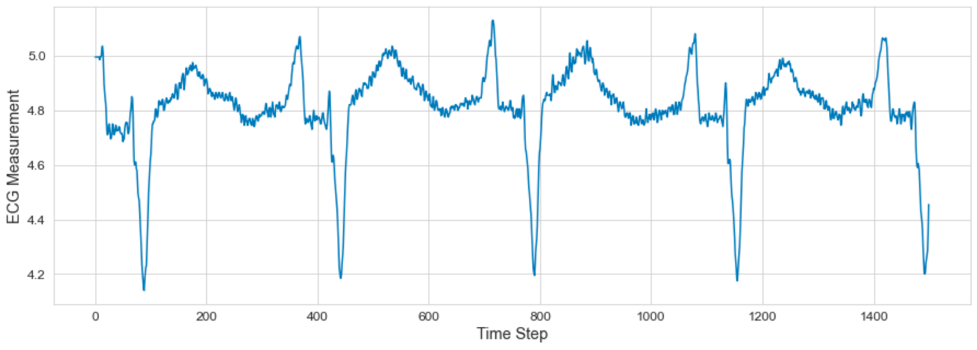
\includegraphics[scale=0.75]{./content/images/4-5.png}
    \caption{Dữ liệu ECG bình thường}
    \label{fig:4-5}
\end{figure}

\begin{figure}[H]
    \centering
    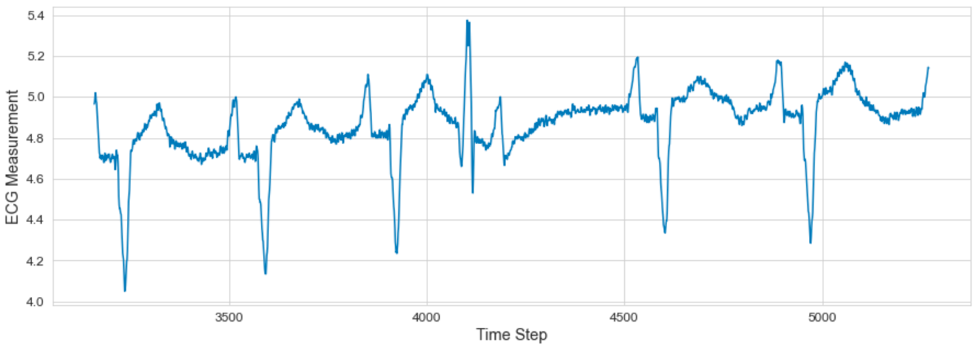
\includegraphics[scale=0.75]{./content/images/4-6.png}
    \caption{Dữ liệu ECG bất thường 1}
    \label{fig:4-6}
\end{figure}

\begin{figure}[H]
    \centering
    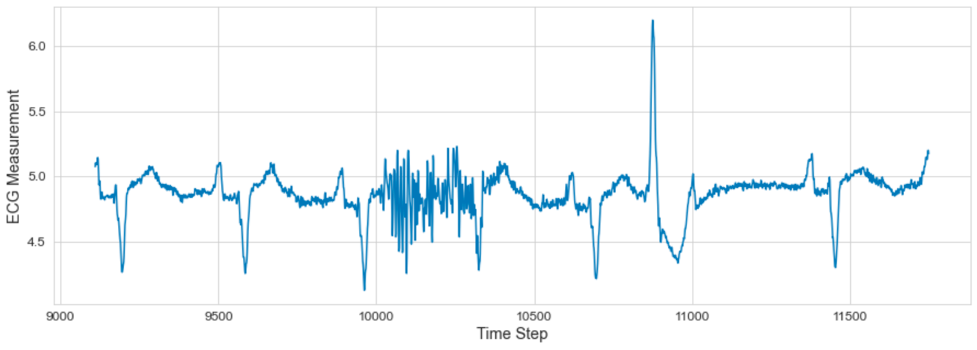
\includegraphics[scale=0.75]{./content/images/4-7.png}
    \caption{Dữ liệu ECG bất thường 2}
    \label{fig:4-7}
\end{figure}

ECG là dữ liệu chuỗi thời gian ghi lại hoạt động của tim, hay còn gọi là điện tâm đồ. Bộ dữ liệu ECG thuộc kho lưu trữ của PhysioBank đã được sử dụng để phát hiện bất thường ở \cite{st12}, \cite{st14}, \cite{st28} và \cite{st29}. Trong nghiên cứu này, chúng tôi sử dụng bộ dữ liệu được sử dụng trong \cite{st12} vì nó cung cấp các dị thường được gắn nhãn do bác sĩ tim mạch chú thích. Có tổng cộng 18000 mẫu dữ liệu với các loại bất thường khác nhau. Hoạt động bình thường của tim được thể hiện trong hình \ref{fig:4-5}. Có 3 điểm bất thường được thể hiện trong hình \ref{fig:4-6} và hình \ref{fig:4-7}.

\subsection{Bộ dữ liệu nhiệt độ máy Numenta}
\begin{figure}[H]
    \centering
    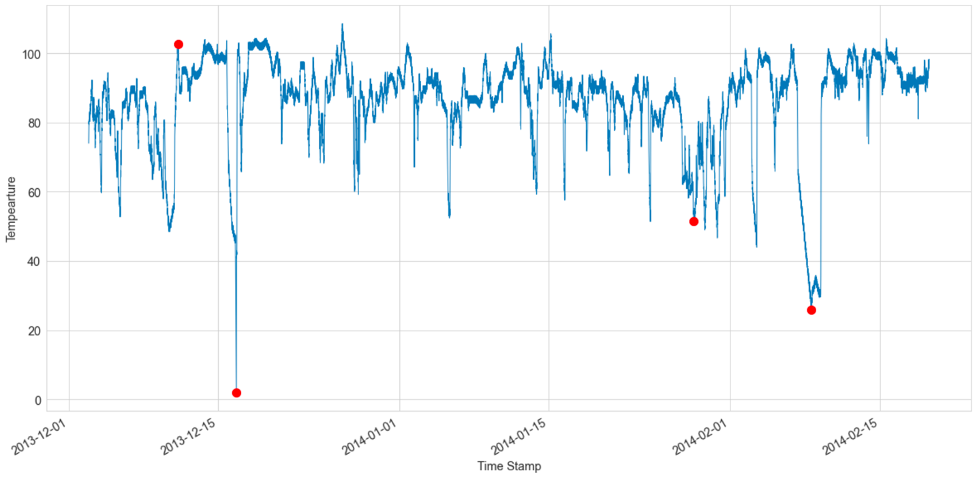
\includegraphics[scale=0.75]{./content/images/4-1.png}
    \caption{Bộ dữ liệu nhiệt độ máy Numenta}
    \label{fig:4-1}
\end{figure}

Bộ dữ liệu được lấy từ \cite{st25}, chứa các giá trị cảm biết nhiệt độ một bộ phận được gắn bên trong một máy công nghiệp lớn. Các giá trị thu thập được trong khoảng thời gian từ tháng 12 năm 2013 đến tháng 2 năm 2014. Có tổng cộng 22695 mẫu dữ liệu, được đo đạc sau mỗi 5 phút. Có bốn điểm bất thường với các nguyên nhân đã biết. Dữ liệu được thể hiện trong hình \ref{fig:4-1}, với các điểm bất thường được biểu thị bằng màu đỏ. Điều bất thường đầu tiên là kế hoạch ngừng hoạt động, và điều thứ tư là một lỗi trong quá trình vận hành. Hai điểm dị thường còn lại không thể nhận biết được bằng mắt thường.

\subsection{Bộ dữ liệu power\_data}
\begin{figure}[H]
    \centering
    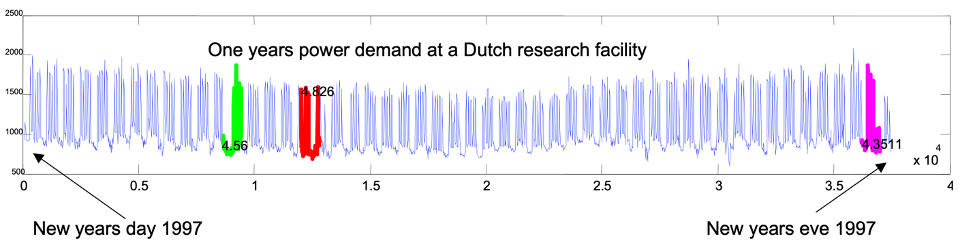
\includegraphics[scale=0.75]{./content/images/4-2.png}
    \caption{Bộ dữ liệu power\_data}
    \label{fig:4-2}
\end{figure}

\begin{figure}[H]
    \centering
    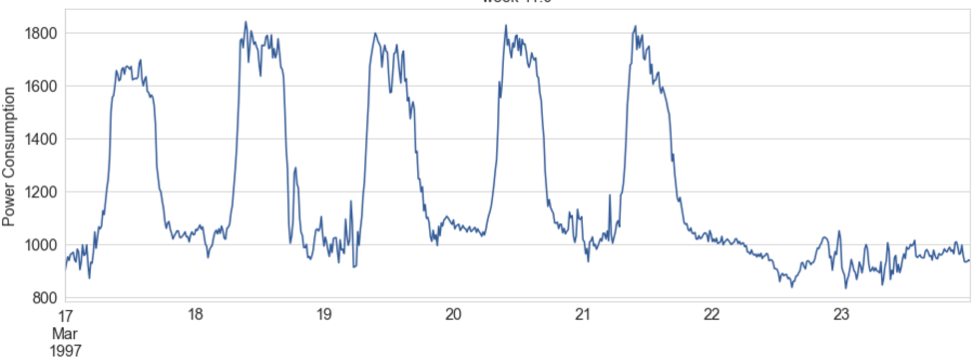
\includegraphics[scale=0.75]{./content/images/4-3.png}
    \caption{Tuần dữ liệu bình thường}
    \label{fig:4-3}
\end{figure}

\begin{figure}[H]
    \centering
    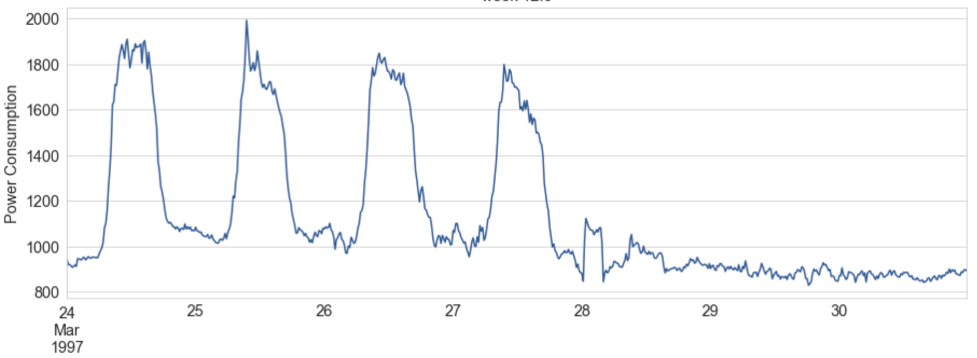
\includegraphics[scale=0.75]{./content/images/4-4.png}
    \caption{Tuần dữ liệu bất thường}
    \label{fig:4-4}
\end{figure}

Bộ dữ liệu được lấy sử dụng trong \cite{st12} \cite{st14} và \cite{st28}, bộ dữ liệu ghi lại nhu cầu điện năng của một cơ sở nghiên cứu tại Hà Lan trong năm 1997 (hình \ref{fig:4-2}). Các mẫu được thu thập sau mỗi 15 phút, cho tổng số 35040 mẫu. Dữ liệu có chu kỳ hàng tuần gồm 672 mẫu với năm mức cao và hai mức thấp tương ứng với mức tiêu thụ điện năng vào các ngày trong tuần và mức tiêu thụ điện năng thấp vào cuối tuần (hình \ref{fig:4-3}). Trong tập dữ liệu này, các ngày trong tuần có nhu cầu điện năng thấp được coi là bất thường, những ngày này có thể rơi vào các ngày lễ (hình \ref{fig:4-4}). Tương tự, những ngày cuối tuần có nhu cầu điện năng cao cũng có thể được coi là bất thường. Chúng tôi sẽ sử dụng cùng một cách tiếp cận này để xác định bất thường.

\subsection{Bộ dữ liệu TEK16}
\begin{figure}[H]
    \centering
    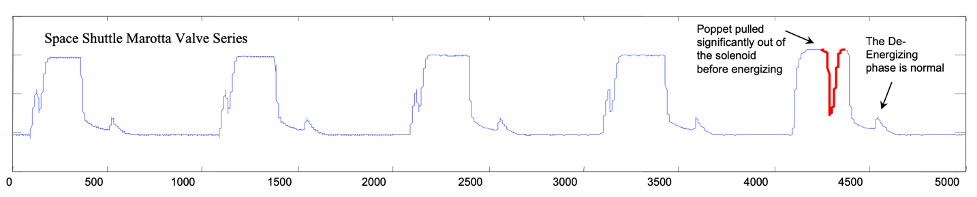
\includegraphics[scale=0.95]{./content/images/4-8.png}
    \caption{Bộ dữ liệu TEK16}
    \label{fig:4-8}
\end{figure}

Bộ dữ liệu TEK16 nằm trong các bộ dữ liệu về nhiên liệu tiêu thụ của phi thuyền. Bộ dữ liệu mô tả mức nhiên liệu đi qua một van của phi thuyền trong một chu kỳ, với các quá trình nạp năng lượng và quá trình xả năng lượng, hình \ref{fig:4-8}. Chúng tôi sử dụng bộ dữ liệu trong \cite{st12}, vì nó có sẵn các điểm bất thường đã được chuyên gia đánh dấu sẵn. Có tổng cộng 5000 mẫu dữ liệu, với mỗi chu kỳ có độ dài 1000 mẫu. Những bất thường trong các quá trình của một chu kỳ sẽ được coi là những điểm dữ liệu bất thường.

\subsection{Bộ dữ liệu chứng khoán stock\_20\_0}
\begin{figure}[H]
    \centering
    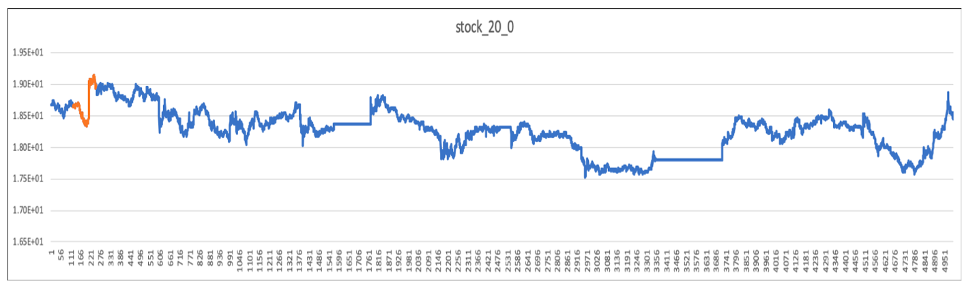
\includegraphics[scale=0.75]{./content/images/4-9.png}
    \caption{Bộ dữ liệu chứng khoán stock\_20\_0}
    \label{fig:4-9}
\end{figure}

Bộ dữ liệu chứng khoán được sử dụng trong \cite{st30}, hình \ref{fig:4-9}. Với 5000 mẫu dữ liệu, và đoạn dữ liệu bất thường đã được đánh dấu sẵn, miêu tả sự thay đổi về giá trị cổ phiếu một cách đột ngột.

\subsection{Bộ dữ liệu memory}
\begin{figure}[H]
    \centering
    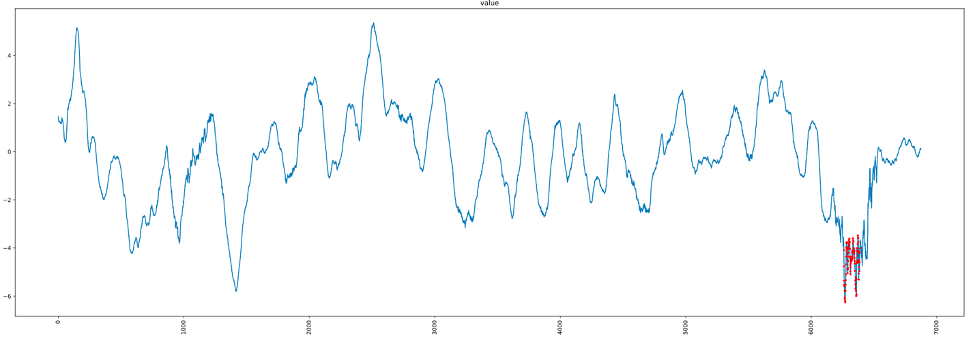
\includegraphics[scale=0.75]{./content/images/4-10.png}
    \caption{Bộ dữ liệu memory}
    \label{fig:4-10}
\end{figure}

Bộ dữ liệu memory được sử dụng trong \cite{st30}, hình \ref{fig:4-10}. Với 6875 mẫu dữ liệu, đoạn dữ liệu bất thường đã được đánh dấu sẵn, miêu tả sự thay đổi về giá trị memory một cách đột ngột và liên tục.

\subsection{Bộ dữ liệu ann\_gun\_CentroidA}
\begin{figure}[H]
    \centering
    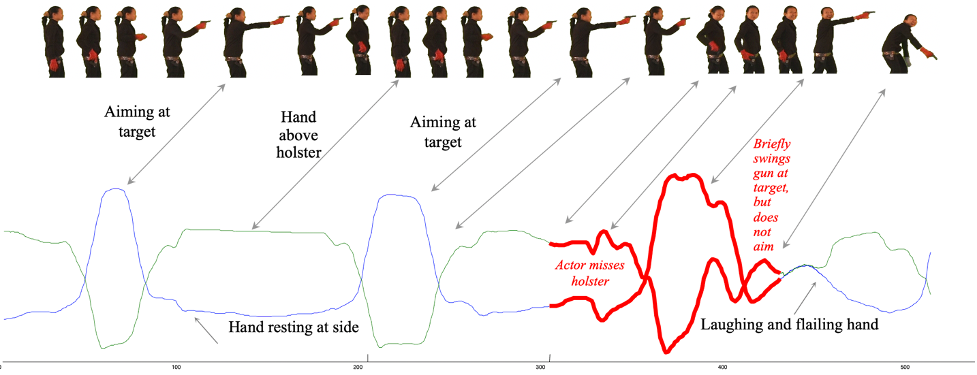
\includegraphics[scale=1]{./content/images/4-11.png}
    \caption{Bộ dữ liệu ann\_gun\_CentroidA}
    \label{fig:4-11}
\end{figure}

Chúng tôi sử dụng bộ dữ liệu trong \cite{st12}, bộ dữ liệu chuỗi thời gian 2D được trích xuất từ một đoạn video về một diễn viên thực hiện các hành động khác nhau có súng và không có súng, hình \ref{fig:4-11}. Hai chuỗi thời gian đo tọa độ X và Y của tay phải các diễn viên. Diễn viên rút một khẩu súng từ một bao da gắn ở hông, nhắm nó vào mục tiêu và trả nó vào bao da. Các nhà nghiên cứu đã phát hiện ra rằng ở khoảng 10 giây sau khi quay, diễn viên đã bỏ sót bao da khi trả súng. Sau đó diễn viên nhìn về phía kỹ thuật viên video và cười. Đây được xem là những điểm dữ liệu bất thường.

\section{Đề xuất mô hình}
Mục tiêu nghiên cứu của đề tài này là xây dựng một mô hình phát hiện chuỗi con bất thường dựa trên phương pháp dự báo với độ sai số nhỏ nhất bằng kỹ thuật học sâu, hình \ref{fig:4-12}. Với sự phát triển của phần cứng trong một thập kỷ qua, các kỹ thuật học sâu đã chứng tỏ được khả năng của mình trong nhiều bài toán phức tạp của cuộc sống. Trong đó, RNN với thiết kế để xử lý dữ liệu dạng chuỗi, thể hiện được sự tương hỗ của dữ liệu được áp dụng thành công vào nhiều bài toán như dịch máy, nhận diện giọng nói, chuyển đổi chữ thành giọng nói và ngược lại,.... và LSTM được dùng để khắc phục nhược điểm đối với dữ liệu phụ thuộc xa trong RNN.

Với những tiềm năng đầy hứa hẹn của các mạng nơ-ron học sâu, trong nghiên cứu này chúng tôi sẽ áp dụng ưu thế của mạng nơ-ron học sâu trong bài toán dự báo, và dựa vào đó để phát hiện chuỗi con bất thường trên các bộ dữ liệu chuỗi thời gian. Các bộ dữ liệu của bài toán này được sưu tầm từ các công trình đi trước, bao gồm về y khoa, dữ liệu doanh nghiệp, công nghiệp...với chiều dài khác nhau, và các bộ dữ liệu này đã được đánh dấu chuỗi con bất thường bởi các nhà nghiên cứu đi trước. Trong tất cả các kịch bản thực nghiệm, độ dài của chuỗi con bất thường được chọn cố định cho mỗi bộ dữ liệu theo gợi ý của các chuyên gia.

Để giải quyết được bài toán đề ra, chúng tôi xây mô hình học sâu, trọng tâm sẽ sử dụng LSTM, vì các bộ dữ liệu đều có sự tương quan giữa giá trị lịch sử tới giá trị hiện tại. Kế thừa nghiên cứu của Malhotra và các cộng sự \cite{st14}, chúng tôi sẽ xây dựng mạng LSTM xếp chồng cho bài toán dự báo và sử dụng giải thuật phân phối sai số dự báo cho bài toán phát hiện chuỗi con bất thường. Bên cạnh đó, \textit{kỹ thuật dự báo nhiều bước} (multi - step ahead prediction) cũng sẽ được chúng tôi áp dụng để tăng tính hiệu quả cho bài toán dự báo.

Sau khi đã có được dữ liệu dự báo, chúng tôi tiến hành tính toán sai số của dữ liệu dự báo với dữ liệu thực tế. Và sai số này sẽ được sử dụng cho bước phát hiện bất thường, chúng tôi sẽ nói rõ phần này trong mục kế tiếp.

\begin{figure}[H]
    \centering
    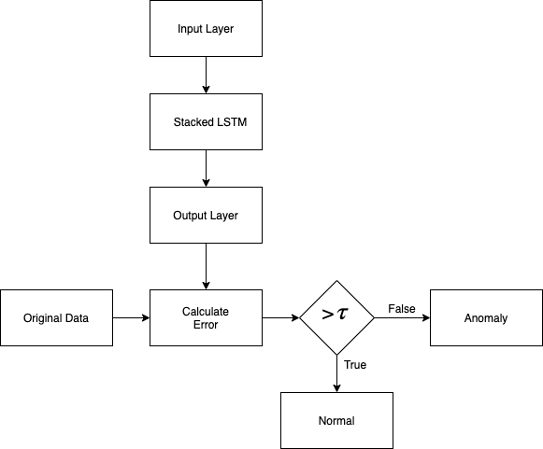
\includegraphics[scale=1.27]{./content/images/4-12.png}
    \caption{Kiến trúc mô hình đề xuất}
    \label{fig:4-12}
\end{figure}

\section{Phương pháp phát hiện bất thường}
Thuật toán phát hiện bất thường được sử dụng trong nghiên cứu bao gồm hai bước chính. Đầu tiên, một mô hình dự báo xây dựng để học các dữ liệu chuỗi thời gian bình thường và dự báo dữ liệu chuỗi thời gian trong tương lai. Sau đó, phát hiện bất thường được thực hiện bằng cách tính toán điểm bất thường từ các lỗi dự báo.

\subsection{Dự báo dữ liệu}
Chúng tôi sử dụng mạng LSTM xếp chồng làm mô hình dự báo. Mô hình nhận đầu vào với \textit{p} giá trị trong quá khứ gần đây nhất và đầu ra là \textit{q} giá trị trong tương lai. Để tiện trong việc diễn giải, chúng tôi gọi \textit{lookback} và \textit{lookahead} tương ứng với \textit{p} giá trị đầu vào và \textit{q} giá trị đầu ra. Mô hình bao gồm các tầng LSTM xếp chồng liên tiếp và được kết nối đầy đủ. Số tầng và số nốt LSTM trong mỗi tầng khác nhau cho mỗi bộ dữ liệu. Để tránh tình trạng quá khớp, tầng \textit{hệ số học} (dropout) được sử dụng giữa các tầng với nhau. tầng đầu ra là một tầng kết nối đầy đủ. Số lượng tế bào thần kinh trong tầng đầu ra bằng giá trị bằng 1, với một tế bào thần kinh cho một giá trị tương lai được dự đoán. Ở đây, chúng tôi sử dụng kỹ thuật dự báo nhiều bước, với số bước tương ứng với giá trị \textit{lookahead}. Kỹ thuật dự báo nhiều bước được chúng tôi lựa chọn là kỹ thuật hồi quy. Ngoài ra, chúng tôi sử dụng hàm kích hoạt tuyến tính trong tầng đầu ra và \textit{MSE} làm hàm mất mát. Mô hình dự báo chỉ được huấn luyện trên dữ liệu bình thường mà không có bất kỳ sự bất thường nào, để mô hình học được hành vi bình thường của dữ liệu chuỗi thời gian.

Thông qua việc sử dụng kỹ thuật dự báo nhiều bước, với giá trị \textit{lookahead} của \textit{q} tại thời điểm \textit{t}, mô hình sẽ dự báo \textit{q} giá trị kế tiếp của chuỗi dữ liệu thời gian, ví dụ \textit{t}+1, \textit{t}+2 ..., \textit{t}+\textit{q}. Chúng tôi sử dụng kỹ thuật dự báo nhiều bước với những mục đích sau:

\begin{enumerate}
\item Chứng tỏ khả năng của mạng nơ-ron học sâu LSTM trong dự báo dữ liệu chuỗi thời gian.
\item Dự báo nhiều bước cung cấp một cách sớm hơn các hành vi trong tương lai, thậm chí các dấu hiệu về sự bất thường.
\item Dự báo nhiều bước tiết kiệm chi phí trong công tác dự báo. Để có được một chuỗi dữ liệu dự báo với \textit{q} bước, thay vì phải chuẩn bị \textit{q} chuỗi dữ liệu đầu vào trong dự báo một bước, thì đối với dự báo nhiều bước, chúng tôi chỉ cần chuẩn bị một chuỗi dữ liệu đầu vào. Điều này có ý nghĩa rất quan trọng trong công tác phát hiện bất thường.
\end{enumerate}

Xét một chuỗi thời gian với tần suất lấy mẫu là 5 phút/1 mẫu. Dự báo 6 bước thời gian trong tương lai sẽ cho biết hành vi trong 30 phút tiếp theo. Nếu có điều gì đó bất thường, ví dụ: một giá trị có độ lớn bất thường, một cảnh báo sớm có thể được đưa ra. Tuy nhiên, dự báo nhiều bước cũng phải đánh đổi với độ chính xác của dự báo.  Trong các thử nghiệm, chúng tôi chỉ sử dụng dự báo nhiều bước khi sai số dự báo ở mức chấp nhận được.

\subsection{Phát hiện bất thường}
Việc phát hiện bất thường được thực hiện bằng cách sử dụng các lỗi dự báo để phát hiện bất thường. Lỗi dự báo, hoặc sai số dự báo là sự khác biệt giữa giá trị dự đoán được đưa ra và giá trị dữ liệu thực tế tại thời điểm \textit{t}. Các sai số dự báo từ dữ liệu huấn luyện được mô hình hóa bằng cách sử dụng phân phối Gauss. Các tham số của Gauss, giá trị giá trị trung tâm hay gọi là trung bình $\mu$ và phương sai $\sigma^{2}$ (hoặc độ lệch chuẩn $\sigma$), được tính bằng cách sử dụng \textit{maximum likelihood estimation} (MLE). Khi đó hàm \textit{mật độ xác suất} (Probability Densities) của sai số dự báo có dạng:

\begin{equation}
\label{eq:23}
P(x) = \frac{1}{{\sigma \sqrt {2\pi } }}e^{{{ - \left( {x - \mu } \right)^2 } \mathord{\left/ {\vphantom {{ - \left( {x - \mu } \right)^2 } {2\sigma ^2 }}} \right. \kern-\nulldelimiterspace} {2\sigma ^2 }}}
\tag{23}
\end{equation}

Trên dữ liệu mới, để tránh \textit{vấn đề triệt tiêu} (vanishing problem) khi giá trị quá nhỏ, \textit{log của mật độ xác suất} (logPD) của sai số dự báo được tính toán và sử dụng làm giá trị để phát hiện bất thường, với các giá trị thấp cho thấy khả năng dữ liệu là bất thường cao hơn. Một tập dữ liệu kiểm thử có chứa cả dữ liệu bình thường và bất thường được sử dụng để xác định giá trị ngưỡng trên các giá trị logPD và có thể tách các điểm dữ liệu bất thường khỏi các điểm dữ liệu bình thường và tạo ra càng ít cảnh báo sai càng tốt. Một tập dữ liệu kiểm tra được sử dụng để phát hiện bất thường với giá trị ngưỡng vừa học được trên tập kiểm thử.

\subsection{Các giả định}
Giả định chính mà chúng tôi đưa ra là một mô hình dự báo được huấn luyện trên dữ liệu bình thường sẽ học các mẫu dữ liệu chuỗi thời gian bình thường. Khi mô hình được sử dụng để dự báo trên dữ liệu mới, mô hình sẽ có sai số dự báo cao hơn trên các vùng có dữ liệu bất thường so với các vùng bình thường. Điều này sẽ cho phép chúng tôi sử dụng các giá trị logPD của lỗi dự báo để xác định bất thường và thiết lập giá trị ngưỡng để tách các điểm dữ liệu bất thường khỏi các điểm dữ liệu bình thường. Một giả thiết khác là sai số dự báo tuân theo phân phối Gauss.

\subsection{Các bước của giải thuật}
Mạng LSTM xếp chồng được huấn luyện trên dữ liệu bình thường và được thiết lập những thông số để tối ưu hoá độ chính xác của dự báo. Với mục đích này, mỗi bộ dữ liệu được chia thành bốn tập dữ liệu con như bước tiền xử lý dữ liệu:

\begin{itemize}
\item Tập huấn luyện \textit{N}, chỉ chứa các giá trị bình thường, dùng cho huấn luyện mô hình.
\item Tập kiểm thử 1 $V_{N}$, chỉ chứa các giá trị bình thường, dùng để đánh giá mô hình trong quá trình huấn luyện.
\item Tập kiểm thử 2 $V_{A}$, chứa các giá trị bình thường và bất thường, dùng để xác định giá trị ngưỡng.
\item Tập kiểm tra \textit{T}, chứa các giá trị bình thường và bất thường, dùng để phát hiện bất thường. 
\end{itemize}

Các bước của giải thuật phát hiện bất thường được tiến hành như sau:

\begin{itemize}
\item Tập huấn luyện \textit{N} được dùng để huấn luyện mô hình. Chúng tôi tiến hành thử nghiệm trên nhiều bộ thông số khác nhau của mô hình LSTM xếp chồng, để tìm bộ thông số thích hợp nhất cho mỗi bộ dữ liệu, và mang lại độ chính xác tốt nhất.
\item Tập kiểm thử 1 $V_{N}$ được sử dụng trong quá trình huấn luyện, để dừng sớm quá trình huấn luyện và nhằm hạn chế tình trạng quá khớp.
\item Dự báo dữ liệu trên tập huấn luyện \textit{N}, sai số giữa giá trị dự báo và giá trị thực tế được mô hình hoá bằng cách sử dụng phân phối Gauss, MLE được dùng để ước lượng giá trị trung tâm hay gọi là trung bình $\mu$ và phương sai $\sigma^{2}$ (hoặc độ lệch chuẩn $\sigma$).
\item Dự báo dữ liệu trên tập kiểm thử 2 $V_{A}$ bằng mô hình LSTM đã được huấn luyện. Giá trị trung bình $\mu$ và phương sai $\sigma^{2}$ đã ước lượng được sử dụng để tính toán giá trị logPD của sai số dự báo trên tập dữ liệu $V_{A}$. Một giá trị ngưỡng được thiết lập để có thể tách biệt các điểm dữ liệu bất thường, với càng ít cảnh báo sai càng tốt.
\item Giá trị ngưỡng đã được xác định từ tập $V_{A}$ được dùng để xác định các bất thường cho sai số của giá trị dự báo trên tập kiểm tra \textit{T}.
\end{itemize}